\documentclass[../report.tex]{subfiles}
\begin{document}	
	
\chapter{Fabrication}
To test the \gls{tpr} it is necessary to design auxiliary components like grating couplers (\gls{te} \& \gls{tm}), tapers, \gls{pbs}. The gratings are designed in way to couple \gls{te} and \gls{tm}-modes from the LASER to the waveguide taper. The tapers are connected to the \gls{tpr}, to direct the light into it. Finally, a \gls{pbs} is designed which again decouples the \gls{te} and \gls{tm}-modes to the grating couplers via tapers where a photo-detector measures the intensity of output modes.  

\begin{figure}[H] %h
	\centering
	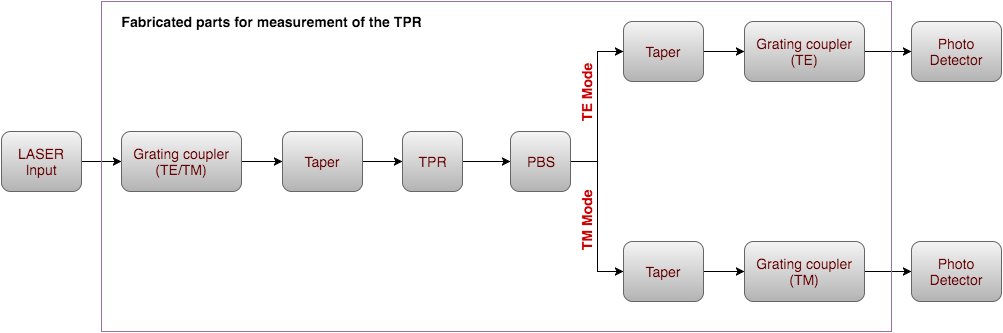
\includegraphics[width=1\textwidth]{4-sys-design}
	\caption{System level block diagram of the fabricated device}
	\label{fig:4_sys_design}
\end{figure}

\section{Unit tests}
Unit Test
Same strategy as Software unit test\\
1. Test if a normal waveguide with TE-TE grating is working with taper.\\
2. Test if a normal waveguide with TE-TM grating is working with taper.\\
3. Test if a normal waveguide with TM-TE grating is working with taper.\\
4. Test if a normal waveguide with TM-TM grating is working with taper.\\
4. Test if a normal waveguide with PBS TE/TM-TM/TE grating is working with taper.\\
5. Test if PR waveguide works with PBS and TE/TM grating for different lengths with taper.\\
6. Check if a normal cantilever is working and it does not stick.\\
7. Check actuation using separation strategy.\\

\section{Fabrication process}\label{sec:fab_process}
The \gls{mems} tunable device was fabricated using a standardized two step dry etch process on \gls{soi} for the silicon device layer (resulting in two heights) and a wet $SiO_2$ under-etch \cite{errando-herranz_low-power_2015}. The first lithography step defines the asymmetric shape of the ridge waveguides in the bus waveguide and the \gls{mems} coupling waveguide, which form a slot waveguide. The second lithography step and the wet under-etch define the free standing cantilever in the \gls{mems} coupling waveguide. The cantilever is delimited by the fully etched slot waveguides, and its free suspended area is determined by the placement of etch holes. The details of the fabrication process steps are described in the following section.

\begin{figure}[H] %h
	\centering
	\includegraphics[width=1.0\textwidth]{4-fabrication}
	\caption{Fabrication process}
	\label{fig:4_fabrication}
\end{figure}

% The fabrication process starts with a clean SOI chip with a \SI{220}{\nano \meter} crystalline silicon device layer and \SI{2}{\micro \meter} buried oxide (\ref{fig:4_fabrication} A). This is a standard substrate specification used by the Epixfab silicon photonics foundries. Electron beam patterning of a \SI{50}{\nano \meter} layer of a high-resolution negative electron beam resist (\gls{hsq}) defines the waveguide structures (\ref{fig:4_fabrication} B). The pattern is then transferred to the device layer by timed dry etch of silicon, resulting in ridge waveguide structures with \SI{110}{\nano \meter} height on a \SI{110}{\nano \meter} thick silicon slab ((\ref{fig:4_fabrication} C)). The patterned \gls{hsq} remains on the chip for the next lithography step.
%$\chem{H_2} + (1/2)\,\chem{O_2} = \chem{H_2O}$

\subsection{Piranha bath}			
Piranha solution is a mixture of sulfuric acid ($\chem{H_2SO_4}$) and hydrogen peroxide ($\chem{H_2O_2}$), used to clean organic residues off substrates. Because the mixture is a strong oxidizing agent, it will remove most organic matter, and it will also hydroxylate most surfaces (add OH groups), making them highly hydrophilic (water-compatible) \cite{piranha_bath}. The fabrication process starts with cleaning the \gls{soi} chip with \SI{220}{\nano \meter} crystalline silicon device layer and \SI{2}{\micro \meter} buried oxide, in the piranha solution (\ref{fig:4_fabrication} A).
 
\subsection{HSQ spin}
A \gls{hsq} resist (negative) is applied on the silicon layer to create a depth of \SI{50}{\nano \meter}. This is achieved by spinning the chip on a  rotating platform at 4000rpm for 30 seconds. The \gls{hsq} layer is hardened by baking the chip in oven at $\chem{170^{\circ}}$ C for 5 minutes. To measure the sample a scratch is made on the chip (on \gls{hsq} layer where there is no design) and checked for depth variations using mechanical profilometer (KLA-Tencor). This is done to verify the profile depth of the mask.

\subsection{First e-beam exposure}
To develop the chip, selective portions of the chip are exposed using e-beam. E-beam exposure exceeds patterning capability of optical lithography and create patterns in sub-microns range. Before loading the chip into the chamber via the sample stage, pressure is adjusted with the external environment. Initially, one corner of the chip is scratched to align the chip and find particles on the chip to focus the beam aperture correctly, to avoid proximity effect (electron deflection) due to astigmatism. Write-field alignment is a very central adjustment in the process of getting the best possible e-beam lithographic result. It is the adjustment of the electromagnetic/electrostatic deflections system inside the column to the high precision X-Y-Z stage. The stage is considered to be "correct" and the e-beam deflection system is aligned to it. To increase the dose in certain portions of the chip (CAD drawn using Raith 150 e-beam lithography software), the scanning speed is slowed down so that more electrons can strike the \gls{hsq} surface and make it harder. Before moving the stage to the Faraday cup it is very good practice to store the current position. It is the position where the Write-Field alignment was made and is required in later exposure steps. The chip is developed using ma-D 525 (micro-resist) which dissolves non-hardened \gls{hsq}. The chip is then put in water to dissolve ma-D 525 and dried using nitrogen. Finally, the exposed \gls{hsq} in the chip is hardened more by putting it in an oven for 40 minutes at $\chem{400^{\circ}}$ C. The chip is cleaned and covered with ceramic glass which avoids formation of dust cloud. After this step the chip resembles the diagram in Fig. \ref{fig:4_fabrication} C. Again mechanical profilometer is used to verify the depth of \gls{hsq}.    

\subsection{First dry etch step}
The device pattern is finally transferred to the device layer by timed dry etch of silicon, resulting in ridge waveguide structures with \SI{110}{\nano \meter} height on a \SI{110}{\nano \meter} thick silicon slab ((\ref{fig:4_fabrication} D)). The pattern is transferred to the device layer by timed dry etch of silicon, resulting in ridge waveguide structures with \SI{110}{\nano \meter} height on a \SI{110}{\nano \meter} thick silicon slab ((\ref{fig:4_fabrication} D)). The patterned \gls{hsq} remains on the chip for the next lithography step. Initially the dry etch chamber is seasoned with a seasoning wafer. After that, chlorine ions and Hydrogen Bromide ($\chem{H^{+}, Br^{-}}$) ions are used to etch silicon in a time controlled chamber. Finally, optical profiling is performed to find out the depth of the silicon etch. This process marks the end of first step lithography process.

\subsection{ZEP7000 spin}
A ZEP7000 resist (positive) is applied on the chip from Fig. \ref{fig:4_fabrication} D using an eppendorf pipette. To achieve a ZEP profile of \SI{200}{\nano \meter} thickness the spinning platform is rotated at 3000 rpm for 45 seconds (depending on the viscosity). The sample is baked at $\chem{175^{\circ}}$ for 3 minutes to make the ZEP layer harder. After this a scratch is made in the sample and the profile depth is measured using a mechanical profilometer (KLA-Tencor).

\subsection{Second e-beam exposure}
Before the second e-beam exposure local axis alignment is performed. This is needed in the second e-beam exposure as it is necessarily to know exactly where the mask should be softened in accordance with the previous e-beam step with \gls{hsq}. Some unique and easily recognizable feature like plus symbol is selected as a mark in the sample. The contamination dots from the focusing is a good example. These are positioned in the center of the screen. The magnification corresponding to the write-field size is selected on the lithography computer and the setting is transferred to the SEM computer \cite{write_field}. Write-field alignment is performed in all the cells manually for dimensional precision. Since ZEP is a positive resist, the exposed portions are developed using p-Xylene solvent and MIBK base. After developing the chip the structure representation looks like Fig. \ref{fig:4_fabrication} E in the fabrication process.

\subsection{Second dry etch step}

\subsection{Wet etching and critical point drying}

%Isopropanol ($\chem{CH_3CHOHCH_3}$)


\section{Final product}

Show SEM image

\end{document}
